
% --------------------------------------------------------------%
% Modelo para trabalho de disciplina do MEEC - UCPEL            %
% Autor: Rogério Albandes                                       %
% Versão: 1.1.3                                                 %
% Data: 01 de março de 2025                                     %
%                                                               %
% Baseado na classe abntex2: https://www.abntex.net.br/         %
% --------------------------------------------------------------%

\documentclass[
	% -- opções da classe memoir --
	article,			% indica que é um artigo acadêmico
	12pt,				% tamanho da fonte
	oneside,			% para impressão apenas frente. Oposto a twoside
	a4paper,			% tamanho do papel. 
	% -- opções da classe abntex2 --
	%chapter=TITLE,		% títulos de capítulos em letras maiúsculas
	%section=TITLE,		% títulos de seções em letras maiúsculas
	%subsection=TITLE,	% títulos de subseções em letras maiúsculas
	%subsubsection=TITLE % títulos de subsubseções em letras maiúsculas
	% -- opções do pacote babel --
	english,			% idioma adicional para hifenização
	brazil				% o último idioma é o principal do documento
	]{abntex2}
\usepackage{newtxtext,newtxmath}    % fonte Times New Roman
\usepackage[T1]{fontenc}            % codificação dos caracteres no PDF
\usepackage[utf8]{inputenc}         % codificação do arquivo
\usepackage{graphicx}               % inclusão de figuras
\usepackage[alf,num]{abntex2cite}   % Para autor-data (alfabética) e citações ABNT sistema numérico
\usepackage{indentfirst}            % indentar 1o. parágrafo
\usepackage{parskip}                % espaço entre parágrafos
\usepackage{microtype} 			    % para melhorias de justificação
\usepackage{color}
\usepackage[section]{placeins}      % comando \FloatBarrier
\usepackage{amsmath}
\usepackage{enumitem}
\usepackage{caption, subcaption}
%\usepackage{natbib}
%\usepackage[authoryear]{natbib}     % Ativa a citação no formato autor-ano.
%\usepackage[authoryear,square]{natbib} % Ativa a citação no formato autor-ano e adiciona colchetes.
\usepackage[alf]{abntex2cite}  % Configuração para autor-data (alfabética)
\usepackage{lipsum}  % Para gerar texto de exemplo
\usepackage{tocbibind} % Garante que "Anexos" apareça no sumário corretamente

\titulo{Título do Trabalho}
\autor{Nome do Autor 1 \and Nome do Autor 2}


% Títulos de capítulos, seções etc. em fonte serifada
\renewcommand{\ABNTEXchapterfont}{\rmfamily}

% -------------------------
% Formatação de referências
% -------------------------
\citebrackets[]
\makeatletter
\renewcommand{\@biblabel}[1]{[#1]\quad}
\makeatother
\AtBeginDocument{\citeoption{abnt-emphasize=bf}}
\renewcommand{\citeonline}[1]{\citeauthoronline{#1} \cite{#1}}
% ---


% --------------------
% Configurações do PDF
% --------------------
\makeatletter
\hypersetup{
    pdftitle={\@title}, 
    pdfauthor={\@author},
    pdfsubject={},
    pdfcreator={LaTeX with abnTeX2},
    pdfkeywords={}, 
    colorlinks=true,    % false: boxed links; true: colored links
    linkcolor=black,    % color of internal links
    citecolor=black,    % color of links to bibliography
    filecolor=black,    % color of file links
    urlcolor=black,
    bookmarksdepth=4
}
\makeatother
% ---

% -------------------------
% Altera as margens padrões
% -------------------------
\setlrmarginsandblock{3cm}{3cm}{*}
\setulmarginsandblock{3cm}{3cm}{*}
\checkandfixthelayout
% ---

% --------------------------------------
% Espaçamentos entre linhas e parágrafos 
% --------------------------------------
% Recuo da primeira linha do parágrafo
\setlength{\parindent}{1.3cm}
% Espaçamento entre um parágrafo e outro:
\setlength{\parskip}{0.2cm}
\OnehalfSpacing                 % espaço entre linhas 1,5
% ---

% Configuração pacote enumitem (itemize, enumerate)
\setlist{parsep=0pt, leftmargin=1.3cm}


%--------------------------
%--------------------------
%--------------------------
% - https://pt.overleaf.com/learn/latex/Code_listing 
\usepackage{xcolor}
\definecolor{codegreen}{rgb}{0,0.6,0}
\definecolor{codegray}{rgb}{0.5,0.5,0.5}
\definecolor{codepurple}{rgb}{0.58,0,0.82}
\definecolor{backcolour}{rgb}{0.95,0.95,0.92}

% --- Json e SQL ------------------------------------------------
\usepackage{listings}
\usepackage{xcolor}

\colorlet{punct}{red!60!black}
\definecolor{background}{HTML}{EEEEEE}
\definecolor{delim}{RGB}{20,105,176}
\colorlet{numb}{magenta!60!black}

\lstdefinelanguage{json}{
    %basicstyle=\normalfont\ttfamily,
    basicstyle=\fontsize{8}{10}\ttfamily,
    %numbers=left,
    numberstyle=\scriptsize,
    stepnumber=1,
    numbersep=8pt,
    showstringspaces=false,
    breaklines=true,
    frame=lines,
    backgroundcolor=\color{background},
    literate=
     *{0}{{{\color{numb}0}}}{1}
      {1}{{{\color{numb}1}}}{1}
      {2}{{{\color{numb}2}}}{1}
      {3}{{{\color{numb}3}}}{1}
      {4}{{{\color{numb}4}}}{1}
      {5}{{{\color{numb}5}}}{1}
      {6}{{{\color{numb}6}}}{1}
      {7}{{{\color{numb}7}}}{1}
      {8}{{{\color{numb}8}}}{1}
      {9}{{{\color{numb}9}}}{1}
      {:}{{{\color{punct}{:}}}}{1}
      {,}{{{\color{punct}{,}}}}{1}
      {\{}{{{\color{delim}{\{}}}}{1}
      {\}}{{{\color{delim}{\}}}}}{1}
      {[}{{{\color{delim}{[}}}}{1}
      {]}{{{\color{delim}{]}}}}{1},
}

\lstdefinelanguage{albandesSQL}{
    language=SQL,
    keywordstyle=\color{blue},
    %basicstyle=\normalfont\ttfamily,
    basicstyle=\fontsize{8}{10}\ttfamily,
    numbers=none,
    numberstyle=\scriptsize,
    stepnumber=1,
    numbersep=8pt,
    showstringspaces=false,
    breaklines=true,
    frame=lines,
    backgroundcolor=\color{background},
    literate=
     *{0}{{{\color{numb}0}}}{1}
      {1}{{{\color{numb}1}}}{1}
      {2}{{{\color{numb}2}}}{1}
      {3}{{{\color{numb}3}}}{1}
      {4}{{{\color{numb}4}}}{1}
      {5}{{{\color{numb}5}}}{1}
      {6}{{{\color{numb}6}}}{1}
      {7}{{{\color{numb}7}}}{1}
      {8}{{{\color{numb}8}}}{1}
      {9}{{{\color{numb}9}}}{1}
      {:}{{{\color{punct}{:}}}}{1}
      {,}{{{\color{punct}{,}}}}{1}
      {\{}{{{\color{delim}{\{}}}}{1}
      {\}}{{{\color{delim}{\}}}}}{1}
      {[}{{{\color{delim}{[}}}}{1}
      {]}{{{\color{delim}{]}}}}{1}
}
\lstdefinelanguage{albandes_json}{
    %basicstyle=\normalfont\ttfamily,
    basicstyle=\fontsize{8}{10}\ttfamily,
    %numbers=left,
    numberstyle=\scriptsize,
    stepnumber=1,
    numbersep=8pt,
    showstringspaces=false,
    breaklines=true,
    frame=lines,
    backgroundcolor=\color{background}
}

% --- Fim Json e SQL -------------------------------
% --- Algoritmo -----------
\usepackage{algcompatible}
% OR \usepackage{algorithmic}
\usepackage{algorithm}
\usepackage{algpseudocode}

\makeatletter
% Reinsert missing \algbackskip
\def\algbackskip{\hskip-\ALG@thistlm}
\makeatother

\usepackage{fixltx2e}
\usepackage{amsmath}
% --- [FIM] Algoritmo -----------
%--------------------------
%--------------------------
%--------------------------

% ----
% Início do documento
% ----
\begin{document}

% Seleciona o idioma do documento (conforme pacotes do babel)
\selectlanguage{brazil}

% Retira espaço extra obsoleto entre as frases.
\frenchspacing

% ----------------------------------------------------------
% ELEMENTOS PRÉ-TEXTUAIS
% ----------------------------------------------------------
\thispagestyle{empty}
\begin{titlingpage}

\begin{figure}[!h]
        \centering
	\vspace{-1cm}
	
\includegraphics[width=0.4\textwidth]{img/logo_UCPEL_SECUNDARIO.pdf}
	\vspace{-1cm}
\end{figure}

\begin{center}\large
    \textsc{Mestrado em Engenharia Eletrônica e Computação}\\
    \textsc{Nome da Disciplina -- Período}\\
    \textsc{Nome do Professor}
    
    \vspace{4.5cm}
    
    
    \vspace{1cm}
   
    {\Huge \textsc{Nome do Trabalho}}
    
    \vspace{4cm}
    
    Nome do Autor 1 \\
    Nome do Autor 2 
    
    \vfill

    \normalsize{Pelotas -- RS\\27 de fevereiro de 2025}

\end{center}

\end{titlingpage}



\begin{resumo}

    Lorem ipsum dolor sit amet, consectetur adipiscing elit. Morbi felis odio, posuere sed porttitor sit amet, vulputate ut nibh. Interdum et malesuada fames ac ante ipsum primis in faucibus. Pellentesque sodales nisi a urna vulputate varius. Duis fermentum felis orci, sit amet dictum sem euismod non. Ut id velit fermentum, venenatis libero vel, pharetra turpis. Donec maximus at nibh pharetra sollicitudin. Cras vitae neque nulla. Morbi pellentesque iaculis orci quis vestibulum. Nulla cursus lectus at neque tincidunt elementum. Aliquam in sodales libero. Quisque commodo sed ante at venenatis. Morbi eu ex sed eros lobortis cursus eu eu metus. Maecenas ut velit malesuada, accumsan mi sed, finibus ante. Sed dapibus aliquet tempus. Cras faucibus purus viverra augue convallis, sed fringilla lectus lobortis.

    \vspace{\onelineskip}
    
    \noindent\textbf{Palavras-chave}: MEEC, UCPEL, Template.
    
\end{resumo}

% --- resumo em inglês ---
\begin{resumo}[Abstract]
\begin{otherlanguage*}{english}
    
    Lorem ipsum dolor sit amet. Sed numquam deserunt sed provident nihil qui accusamus sunt qui ratione neque qui deserunt veritatis sed veritatis sequi et alias libero. Et sequi consequatur ut rerum delectus ex quia quas. Sit beatae dolores eum architecto temporibus nam dolorem eligendi. Est voluptas repellendus eos perferendis molestias et dignissimos ratione nam dicta facilis et voluptatem accusamus eum facilis sint sit repellat suscipit. Sit dicta alias est quis suscipit est voluptates dolorum ut voluptate exercitationem qui tempore molestiae? Et itaque dolorum At amet ipsam est mollitia quia aut dolor internos vel reiciendis molestiae qui eveniet consequatur sed accusantium ipsa.
    
    \vspace{\onelineskip}
    
    \noindent\textbf{Keywords}: MEEC, UCPEL, Template.
\end{otherlanguage*}
\end{resumo}

% Sumário
\tableofcontents*


% ----------------------------------------------------------
% ELEMENTOS TEXTUAIS
% ----------------------------------------------------------
\textual

\section{Introdução}

O uso do \textbf{Overleaf} e do \textbf{LaTeX} é altamente benéfico para alunos de mestrado, especialmente aqueles que precisam produzir dissertações, artigos científicos e relatórios técnicos de alta qualidade. Diferente dos processadores de texto convencionais, o \LaTeX\ permite um controle preciso da formatação, garantindo a correta estruturação de referências, equações matemáticas e tabelas complexas. Além disso, ele segue padrões acadêmicos reconhecidos internacionalmente, facilitando a submissão de trabalhos para conferências e periódicos.  

O Overleaf, por sua vez, é uma plataforma colaborativa baseada em nuvem que simplifica o uso do \LaTeX\, eliminando a necessidade de instalar pacotes localmente. Isso possibilita que alunos e orientadores trabalhem simultaneamente no mesmo documento, facilitando revisões e ajustes em tempo real. Além disso, o Overleaf conta com templates prontos para diversas universidades e publicações científicas, o que agiliza a escrita acadêmica ao reduzir o tempo gasto com ajustes de formatação.  

Outro grande benefício do \LaTeX\ é a sua capacidade de lidar com grandes quantidades de referências bibliográficas por meio do BibTeX. Isso evita problemas comuns em editores de texto tradicionais, como erros na numeração ou inconsistências no estilo de citação. Para alunos de mestrado que precisam integrar diversas fontes de pesquisa e garantir a padronização da bibliografia, essa funcionalidade é essencial.  

Além da qualidade tipográfica superior, o \LaTeX\ também é muito útil para a escrita de documentos técnicos com grande quantidade de fórmulas matemáticas, gráficos e algoritmos. Diferente de editores visuais, que podem apresentar problemas na exibição desses elementos, o \LaTeX\ garante que tudo seja representado corretamente, independentemente do dispositivo ou plataforma onde o documento for aberto.  

Por fim, ao utilizar o Overleaf e \LaTeX\, o aluno de mestrado desenvolve habilidades valiosas para a pesquisa acadêmica e a produção científica, preparando-se melhor para um futuro na academia ou na indústria. O domínio dessas ferramentas proporciona mais eficiência, organização e profissionalismo na apresentação dos trabalhos, tornando-os mais claros e acessíveis para a comunidade científica.





\section{Desenvolvimento}

\subsection{Citações}

    Utilizaremos o formato de citação autor-ano, assegurando a padronização das referências bibliográficas ao longo do documento e facilitando a identificação das fontes citadas no texto.

    Nesta frase, apresentamos um exemplo de citação indireta:

    Segundo \cite{bianchi2021miint}, o uso da técnica X é recomendado por apresentar vantagens significativas, como a melhoria da eficiência computacional e a redução da complexidade na implementação de determinados processos. Essa abordagem tem sido amplamente adotada em diferentes contextos devido à sua eficácia na resolução de problemas específicos. Posteriormente, uma abordagem alternativa foi descrita por pesquisadores em \cite{vadlamudi2023implementing}, os quais propuseram uma metodologia distinta que aprimora determinados aspectos do desempenho e da escalabilidade, possibilitando sua aplicação em cenários mais complexos e exigentes.

    Quando a citação for maior que três linhas, devemos formatá-la como uma citação em bloco, conforme o exemplo a seguir:  

    \begin{citacao}
    Lorem ipsum dolor sit amet, consectetuer adipiscing elit. Ut purus elit, vestibulumut, placerat ac, adipiscing vitae, felis. Curabitur dictum gravida mauris. Nam arcu libero,nonummy eget, consectetuer id, vulputate a, magna. Donec vehicula augue eu neque. \cite{lamnaour2024semantic}
    \end{citacao}

    As referências estão no arquivo \texttt{referencias.bib}, no formato BibTeX. Vários portais de artigos disponibilizam a citação nesse formato, incluindo o próprio Google Scholar. O BibTeX facilita a organização e a padronização das referências bibliográficas, permitindo sua inserção automática no documento.  

    A seguir, estão listados alguns links explicando esse formato e como utilizá-lo corretamente no Overleaf:
    \begin{itemize}
        \item 
        \textbf{Using BibTeX}: Este guia fornece instruções detalhadas sobre como utilizar o BibTeX, incluindo a criação de arquivos \texttt{.bib} e a inserção de referências em documentos LaTeX~\footnote{\url{https://www.bibtex.org/Using/}}; 
        \item 
        \textbf{BibTeX Format Explained [with examples]}: Este artigo explica a estrutura do formato BibTeX, detalhando os tipos de entradas e campos disponíveis, acompanhado de exemplos práticos\footnote{\url{https://www.bibtex.com/g/bibtex-format}}; 
        \item 
        Bibliography Management with BibTeX: O Overleaf oferece um tutorial abrangente sobre como gerenciar bibliografias utilizando BibTeX, abordando desde a criação de arquivos de bibliografia até a configuração de estilos de citação\footnote{\url{https://www.overleaf.com/learn/latex/Bibliography_management_with_bibtex}}.
    \end{itemize}

\subsection{Figuras}

Para incluir figuras, como a Figura~\ref{fig:exemplo-figura}, podemos utilizar formatos comuns de imagens, como JPG ou PNG. Entretanto, dê preferência a figuras vetorizadas, no formato PDF, assim a qualidade não será comprometida e o arquivo PDF final terá um tamanho menor. 

\begin{figure}[!htbp]
    \centering
    \caption{\label{fig:exemplo-figura} Arquitetura de Software do \textit{Middleware} EXEHDA.}
    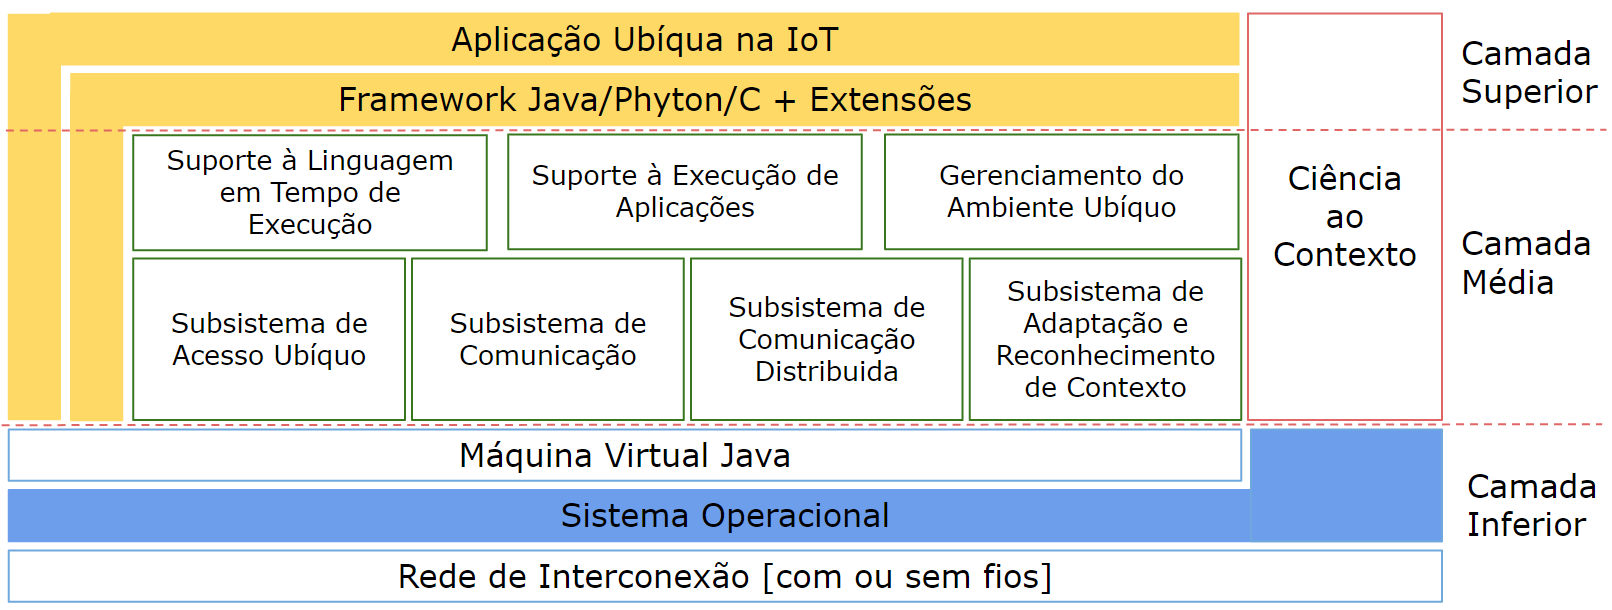
\includegraphics[width=\textwidth]{img/ArquiteturaExehda_v4-pt_BR.png}
    
    \legend{Fonte: Elaborada pelo autor, adaptada de \cite{lopes2014middleware}}
\end{figure}

As figuras no \LaTeX\ nem sempre são posicionadas exatamente onde foram inseridas no código. Em vez disso, o algoritmo interno ajusta automaticamente a disposição dos elementos para garantir a melhor apresentação do documento. Portanto, evite expressões como ``de acordo com a figura abaixo'', pois a figura pode não estar imediatamente abaixo. Em vez disso, utilize referências automáticas, como: ``de acordo com a \autoref{fig:exemplo-figura}''.

Para evitar que um parágrafo seja interrompido por figuras, você pode utilizar o comando \verb|\FloatBarrier|. Caso esteja lidando com várias figuras seguidas e deseje forçar sua exibição antes de prosseguir para a próxima seção do texto, o comando \verb|\clearpage| pode ser útil, garantindo que todas as figuras pendentes sejam renderizadas antes da nova página.

\subsubsection{Figuras em minipages}
\emph{Minipages} são utilizadas para organizar textos, imagens ou outros elementos dentro de quadros com tamanhos e posições controladas. Esse recurso é especialmente útil para alinhar conteúdos lado a lado sem depender da estrutura padrão de colunas. Veja, por exemplo, a \autoref{fig_minipage_imagem1} e a \autoref{fig_minipage_grafico2}.

% \begin{figure}[htb]
%  \label{teste}
%  \centering
%   \begin{minipage}{0.4\textwidth}
%     \centering
%     \caption{Imagem 1 da minipage} \label{fig_minipage_imagem1}
%     
\includegraphics[scale=0.9]{img/abntex2-modelo-img-marca.pdf}
%     \legend{Fonte: Produzido pelos autores}
%   \end{minipage}
%   \hfill
%   \begin{minipage}{0.4\textwidth}
%     \centering
%     \caption{Gráfico 2 da minipage} \label{fig_minipage_grafico2}
%     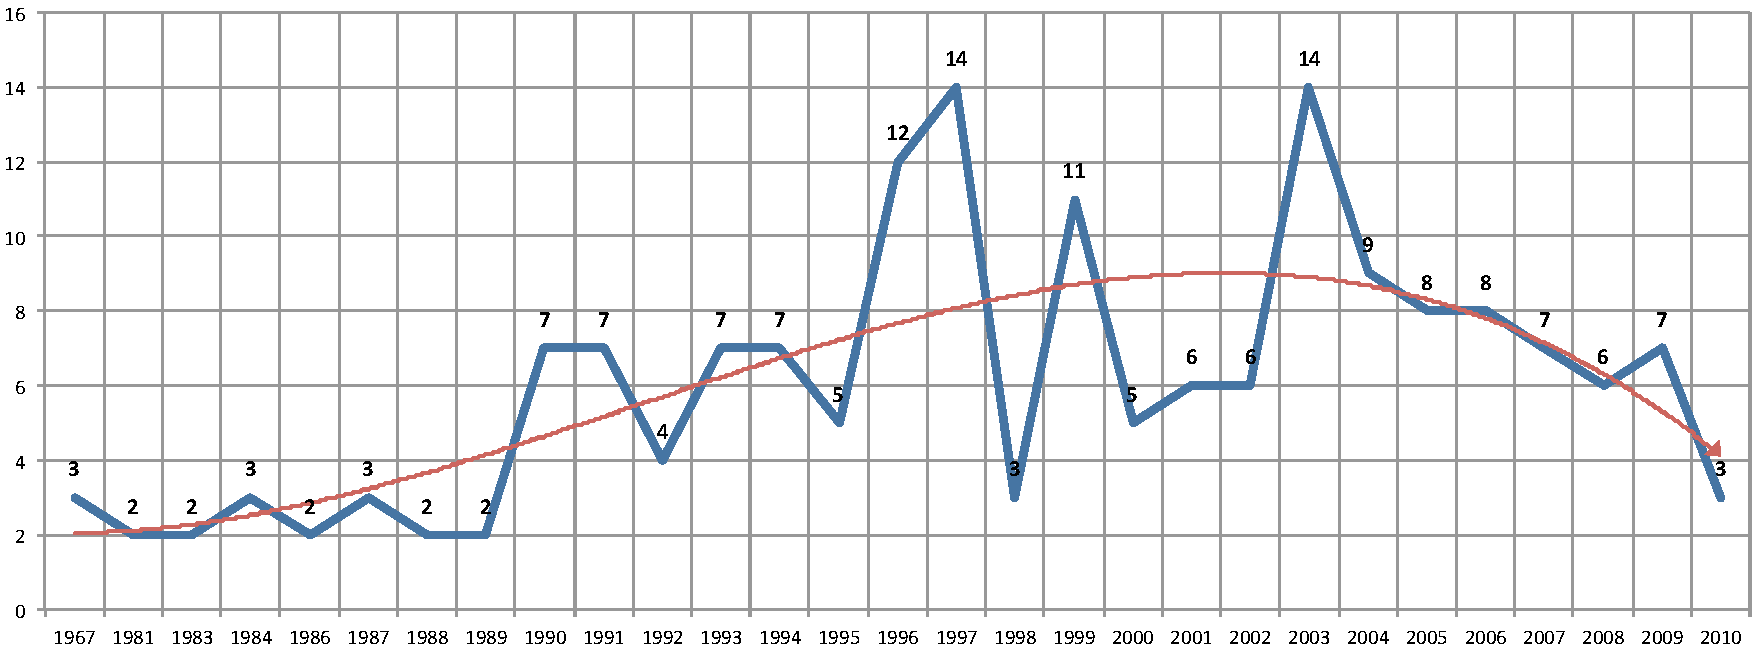
\includegraphics[scale=0.2]{img/abntex2-modelo-img-grafico.pdf}
%     \legend{Fonte: \cite{nunes2011associations} }
%   \end{minipage}
% \end{figure}

\begin{figure}[htb]
 \label{teste}
 \centering
  \begin{minipage}{0.4\textwidth}
    \centering
    \caption{ESP 8266} \label{fig_minipage_imagem1}
    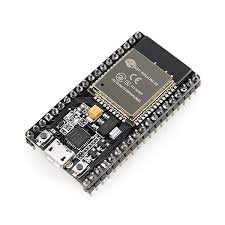
\includegraphics[scale=0.4]{img/esp32.jpeg}
    \legend{Fonte: Produzido pelos autores}
  \end{minipage}
  \hfill
  \begin{minipage}{0.4\textwidth}
    \centering
    \caption{ESP 32} \label{fig_minipage_grafico2}
    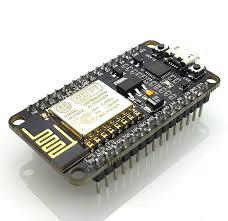
\includegraphics[scale=0.38]{img/esp8266.jpeg}
    \vspace{2mm}
    \legend{Fonte: \cite{nunes2011associations} }
  \end{minipage}
\end{figure}

\subsubsection{Sub-figuras}
Sub-figuras em \LaTeX\ são figuras organizadas dentro de uma figura principal, permitindo que várias imagens sejam apresentadas lado a lado ou empilhadas dentro de um mesmo ambiente, vide figura~\ref{fig:exemplo-subfiguras}. Isso é útil para comparar gráficos, diagramas ou imagens relacionadas sem precisar criar múltiplos ambientes figure.

\begin{figure}[!htbp]
    \centering
    \caption{\label{fig:exemplo-subfiguras} Exemplo de subfiguras.}
    \begin{subfigure}[b]{0.3\textwidth}  % tamanho da subfigura
        \centering
        
\includegraphics[width=\textwidth]{img/logo_UCPEL.png}
        \caption{\label{fig:subfig1} subfigura à esquerda}
    \end{subfigure}
    \hfill
    \begin{subfigure}[b]{0.3\textwidth}  % tamanho da subfigura
        \centering
        
\includegraphics[width=\textwidth]{img/logo_UCPEL_PRETO.png}
        \caption{\label{fig:subfig2} subfigura à direita}
    \end{subfigure}
\end{figure}

\subsection{Tabelas}

Para a criação de tabelas em \LaTeX\, como a~\autoref{tab:gpio} e a~\autoref{tab:algoritmo-compara}, é possível utilizar a ferramenta online \url{https://www.tablesgenerator.com}, que permite elaborar tabelas de forma visual e intuitiva. Essa ferramenta facilita a formatação dos dados, possibilitando a personalização de estilos, alinhamentos e bordas, além de gerar automaticamente o código correspondente em \LaTeX\. Dessa forma, a utilização dessa abordagem simplifica a construção de tabelas complexas, garantindo maior precisão na apresentação dos dados e otimização do tempo na edição do documento.

\begin{table}[!ht]
\centering
\footnotesize
\caption{GPIOS}
%\vspace{5mm}
\label{tab:gpio}
\begin{tabular}{l|l}
\hline
ESP 32      & SIM 800L \\ \hline
GPIO 2 (TX) & RX       \\ \hline
GPIO 4 (RX) & TX       \\ \hline
GND         & GND      \\ \hline
\end{tabular}

\vspace*{3mm}
{\small Fonte: Preparada pelo autor.}     
\end{table}

As tabelas em \LaTeX\ permitem a organização clara e estruturada de dados, oferecendo ampla flexibilidade na formatação, alinhamento e personalização, garantindo uma apresentação precisa e profissional em documentos técnicos e acadêmicos, como ilustrado na \autoref{tab:algoritmo-compara}, onde a disposição dos dados segue um padrão bem definido para facilitar a leitura e interpretação das informações.


\begin{table}[h]
\small
\centering
\captionsetup{justification=centering}
\caption{Comparison of Association Rule Algorithms}
\label{tab:algoritmo-compara}
\begin{tabular}{|l|l|l|l|}
\hline
\textbf{Algorithm} & \begin{tabular}[c]{@{}l@{}}\textbf{Ease} \\ \textbf{Deployment}  \end{tabular} & \begin{tabular}[c]{@{}l@{}}\textbf{Big Data} \\\textbf{Efficiency} \end{tabular} & \begin{tabular}[c]{@{}l@{}}\textbf{Computational } \\ \textbf{Complexity}\end{tabular} \\ \hline
Apriori & High & Medium & High \\ \hline
FP-Growth & Medium & High & Medium \\ \hline
Eclat & Medium & \begin{tabular}[c]{@{}l@{}}Alta\end{tabular} & \begin{tabular}[c]{@{}l@{}}Variável \end{tabular} \\ \hline
RARM & Low & High & High \\ \hline
STUCCO & Low & Medium & High \\ \hline
\end{tabular}

\vspace*{3mm}
{\small Source: Prepared by the author.}        


\end{table}

\subsection{Equações}

Um exemplo de equação destacada pode ser observado na \autoref{eq:exemplo-1}, enquanto um exemplo de equação inserida diretamente no meio do parágrafo é dado por: $v_j(n+1) = v_j(n) + \Delta v_j(n)$ . Caso ainda não esteja familiarizado com a sintaxe matemática do \LaTeX\ ou não conheça o nome exato de um determinado símbolo matemático, é recomendável utilizar a ferramenta online \url{https://editor.codecogs.com} Esse editor permite a construção de equações de forma visual e intuitiva, semelhante ao Editor de Equações do Microsoft Word, facilitando a criação e formatação de expressões matemáticas complexas sem a necessidade de memorizar comandos específicos.

\begin{equation}\label{eq:exemplo-1}
    v_j(n+1) = v_j(n) + \Delta v_j(n) =  v_j(n) - \eta_v\cdot\nabla_{v_j}E(n) = v_j(n) - \eta_v\cdot\frac{\partial E(n)}{\partial v_j(n)}
\end{equation}


% Início dos anexos
%\newpage
%\section{Anexos} % Título opcional para os anexos
% \appendix
% \addcontentsline{toc}{section}{Anexos} % Adiciona "Anexos" ao sumário

% \clearpage % Inicia o primeiro anexo em uma nova página
% \section{Primeiro Anexo}
% \lipsum[3] 
% \clearpage % Inicia o segundo anexo em uma nova página
% \section{Segundo Anexo}
% \lipsum[4] 



% ----------------------------------------------------------
% ELEMENTOS PÓS-TEXTUAIS
% ----------------------------------------------------------
\postextual

% Referências bibliográficas
%\bibliographystyle{apalike} % Estilo de referência autor-ano
%\bibliographystyle{plain}
\bibliographystyle{abntex2-alf}  % Estilo bibliográfico ABNT autor-data
\bibliography{referencias}

\end{document}
